\documentclass[11pt,final,oneside]{fithesis}
\usepackage{czech}
\usepackage[plainpages=false, pdfpagelabels]{hyperref}

% Aby bylo cislovano i subsubsection
\setcounter{secnumdepth}{3}
\setcounter{tocdepth}{3}

%% My packages
\usepackage{url}
\usepackage{ifpdf}
\usepackage{graphicx}



\usepackage{listings}
\lstset{ %
% language=Java,                % choose the language of the code
tabsize=2,                      % sets default tabsize to 2 spaces
captionpos=b,                   % sets the caption-position to bottom
breaklines=true,                % sets automatic line breaking
breakatwhitespace=false,        % sets if automatic breaks should only happen at whitespace
escapeinside={\%*}{*)},          % if you want to add a comment within your code
basicstyle=\ttfamily
}

\renewcommand{\lstlistingname}{Výpis}

\hypersetup{
    colorlinks,%
    citecolor=black,%
    filecolor=black,%
    linkcolor=black,%
    urlcolor=black
}
%\urlstyle{rm}

\thesistitle{Statická analýza jazyka C}
\thesissubtitle{Bakalářská práce}
\thesisstudent{Jan Šťastný}
\thesiswoman{false}
\thesisfaculty{fi}
\thesisyear{jaro 2008}
\thesisadvisor{Mgr. Jan Obdržálek, Ph.D.}

\begin{document}
\FrontMatter
\ThesisTitlePage

\begin{ThesisDeclaration}
\DeclarationText
\AdvisorName
\end{ThesisDeclaration}

\begin{ThesisThanks}
Předně chci poděkovat vedoucímu práce Janu Obdržálkovi za jeho vytrvalou péči a mnohé konzultace.

Dále bych rád poděkoval členům projektu, se kterými jsem mohl spolupracovat, předně potom Jarkovi Novotnému za práci, na kterou mohu navazovat.

Poděkování patří také průmyslovému partnerovi Fakulty informatiky, firmě ANF DATA spol.~s~r.~o., za jejich podporu činnosti laboratoře ITI. Firmě ANF DATA spol.~s~r.~o. také děkuji za stáž, kterou jsem ve firmě strávil v létě 2007. 
\end{ThesisThanks}

\begin{ThesisAbstract}
Hlavním cílem této práce je popsat změny a vylepšení nástroje na statickou analýzu, vyvíjeného v laboratoři ITI. Hlavním úkolem bylo vyvinout a naimplementovat nový static checker, který bude ovládán XML definičními soubory, které jsou pro uživatele lehce čitelné a které může uživatel se základní znalostí informatiky intuitivně napsat. Mezi cíle patří implementace ovládání nástroje z příkazové řádky začlenění logovacího nástroje \textsc{log4j} a implementace grafu volání procedur.
\end{ThesisAbstract}


\begin{ThesisKeyWords}
Statická analýza, C, XML, Java, konečný automat, hledání chyb
\end{ThesisKeyWords}

\MainMatter
\tableofcontents
\chapter{Úvod}
Vývoj software je v dnešní době průmyslem s obrovskými rozpočty. Jedná se o průmysl zaměstnávající mnoho odborníků na celém světě. I přes rozsah prostředků obsahují softwarové produkty mnoho chyb.

 Vývoj každého softwarového produktů prochází různými fázemi. Testování a hledání chyb by mělo být neodlučitelnou fází vývoje každého produktu. Současně se často jedná o jednu z nejméně příjemných fází a o fázi, kterou vývojáři nemají moc v oblibě. Z tohoto důvodu je zde přirozená tendence některých vývojářů tuto fázi opomíjet. Důsledkem jsou potom programy, které nefungují správně. Škála dopadů chyb je velmi široká. Může začínat od relativně banálních chyb, které způsobí, že dialogové okno zapříčiní \uv{zamrznutí} systému na několik okamžiků, až po chyby, které mohou mít za důsledek výpadek serveru, se kterým pracují stovky uživatel na několik minut či hodin.
  
Některé chyby lze nalézt a odstranit relativně rychle a jednoduše (například spuštěním programu v ladícím prostředí a odkrokováním programu), jiné chyby se hledají mnohem složitěji. Příkladem chyb, které se hledají velmi obtížně jsou chyby v částech kódu, který je spouštěn jen zřídka a za složitých podmínek. Takové chyby se těžko reprodukují a tím pádem i těžko odstraňují. Takové chyby se často nacházejí například v ovladačích hardware. Testování je v tomto případě velmi obtížné a často téměř nemožné.

Ideálním řešením je přístup, kdy program není při hledání chyb potřeba spouštět a chyby jsou hledány přímo ve zdrojovém kódu. Odpadá například potřeba mít k dispozici hardware, jehož ovladače máme testovat. Tomuto přístupu se říká statická analýza. Při hledání chyb program není kompilován ani spouštěn. Analýza pracuje přímo se zdrojovým kódem programu bez jeho spustitelné verze.

Tato bakalářská práce popisuje nástroj na statickou analýzu vyvíjený v laboratoři ITI\footnote{ITI = Institut Teoretické Informatiky} na Fakultě informatiky.

V následující kapitole je popsán současný stav nástroje a jeho dělení na moduly. Jsou zde také popsány již implementované checkery.

Třetí kapitola popisuje obecné práce, které jsem na nástroji provedl. Zavedl jsem podporu ovládání programu pomocí argumentů příkazové řádky, do nástroje jsem zabudoval logovací nástroj \textsc{log4j} a vytvořil jsem modul pro tvorbu grafu volání.

Čtvrtá kapitola je detailním popisem nového statického checkeru (\textit{automaton checker}). V této kapitole je mimo jiné kompletně popsán algoritmus analýzy programu.
%  a v jejím závěru jsou obsaženy ukázky XML definičních souborů.

Pátá kapitola práci uzavírá. 
 
\chapter{Popis nástroje}

Ve spolupráci s firmou ANF DATA spol.~s~r.~o., průmyslovým partnerem Fakulty informatiky, je ve laboratoři ITI vyvíjen od roku nástroj na statickou analýzu jazyka C.

\section{Architektura}
Nástroj se člení na jednotlivé moduly. Snahou je, aby jednotlivé moduly byly co nejvíce samostatné. Jednotlivé moduly vzájemně spolupracují. Každý modul má v nástroji většinou svůj vlastní balíček. V této sekci jsou popsány nejdůležitější moduly nástroje.

\begin{figure}[ht]
\begin{center}
\ifpdf
	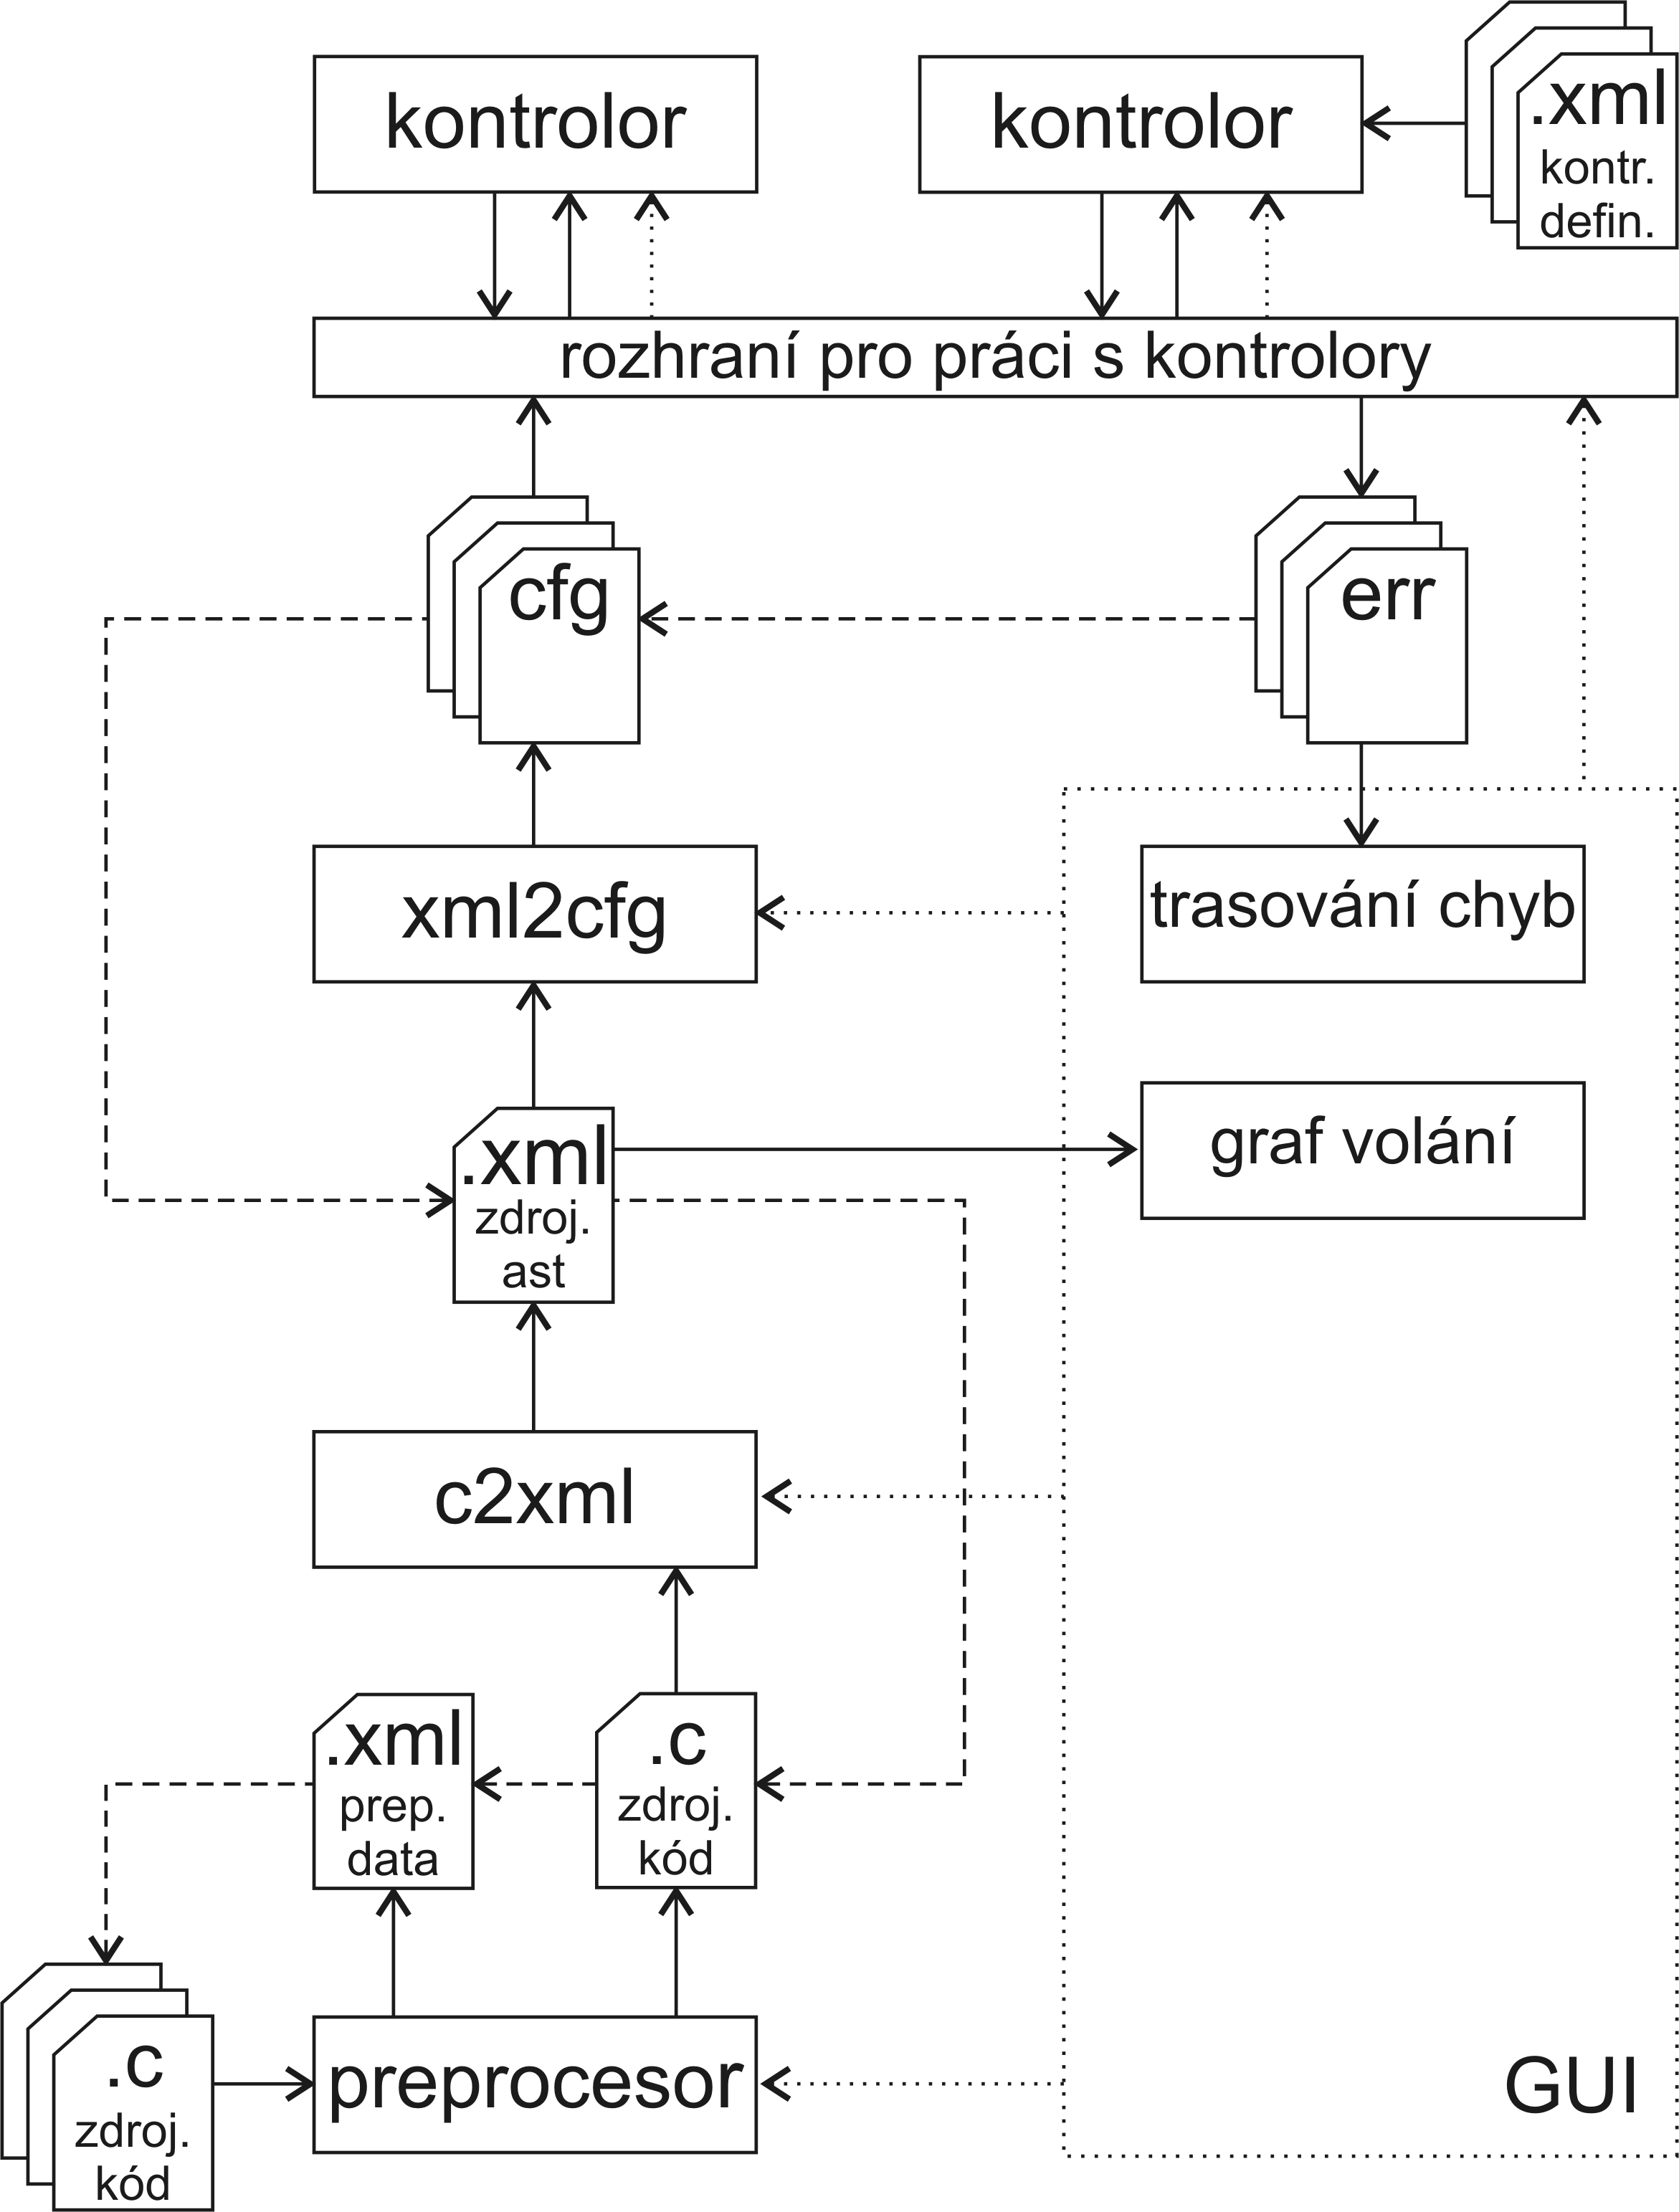
\includegraphics[width=6cm]{img/arch.png}
\fi
\end{center}
\caption{Architektura nástroje}
\label{arch-img}
\end{figure}

\paragraph*{c2xml} Klíčovou komponentou je modul \texttt{c2xml}, který ze vstupního zdrojového kódu v jazyce C generuje abstraktní syntaktický strom (AST), který je na reprezentován ve formátu XML. Výstupní XML dodržuje schéma. Toto schéma je dostupné na adrese \url{http://arran.fi.muni.cz/wiki/index.php/Schema}. Tento modul přijímá zdrojový kód, který je již preprocesován.

\paragraph{xml2cfg} Modul \texttt{xml2cfg} generuje z AST graf toku řízení. Graf toku řízení je generován pro každou funkci zvlášť. Tento graf je přijímán checkery, který jej používají pro analýzu. 

\paragraph{checkery} Nástroj obsahuje více tzv. \textit{checkerů} (na obrázku \ref{arch-img} je pro checkery použit výraz kontrolor). Checker je modul, který hledá ve vstupním zdrojovém kódu určitý typ chyb. Checkery pracují s grafem toku řízení. Pro grafickou reprezentaci chyb je checkerům k dispozici třída \texttt{ErrorForm} v modulu GUI.

V aktuální verzi jsou v nástroji obsaženy tyto checkery:
\begin{itemize}
	\item \textbf{Univerzální statický checker} (nebo podle terminologie použité v diplomové práci Jaroslava Novotného\cite{jarek} také univerzální staticky kontrolor) hledá chyby na základě uživatelem zadaných XML definičních souborů. Tento checker umí hledat např. chyby typu špatného párování zámku. Tento checker obsahuje interprocedurální rozšíření.
	\item \textbf{Kontrolor práce s pamětí} je popsán v diplomové práci Michala Fiedlera\cite{michal} hledá chyby typu \uv{program používá paměť, aniž by zkontroloval její správnou alokaci} nebo \uv{funkce neuvolnila paměť, kterou alokovala}.
	\item \textbf{Automaton checker} je kompletně přepracovaný univerzální statický checker. Jeho detailní popis se nachází v kapitole \ref{automaton-checker}. Checker vyhledává chyby podle definic zadávaných uživatelem ve formátu XML. Schéma definičních XML dokumentů je jednoduchým popisem konečného automatu.
\end{itemize}



%% =================================================================
%%				Obecné práce na nástroji
%% =================================================================
\chapter{Obecné práce na nástroji}

Na vývoji nástroje se v průběhu času vystřídalo více lidí a každý na nástroji udělal svoji část práce. Každý z nich byl ale většinou zaměřen na svoji komponentu a práce na nástroji jako celku někdy zaostávala. Některé chybějící součásti, které jsem naimplementoval popisuji v této kapitole.

%% =================================================================
%%				Command line
%% =================================================================
\section{Podpora argumentů příkazové řádky}\label{toc-command-line}
\subsection{Motivace}
Nástroj sice obsahuje propracované grafické uživatelské rozhraní. To ale není vhodné například pro dávkové testování souborů nebo pro automatické spouštění nástroje jinými programy (např. pro plánované spouštění nástrojem \textsc{make}). Ovládání pomocí argumentů příkazové řádky přijde vhod také při testování a ladění nástroje kdy chce programátor např. pokaždé otevřít stejný zdrojový soubor a spustit na něm stejný kontrolor.

\subsection{Implementace}
Pro jazyk Java existuje více knihoven pro zpracování argumentů příkazové řádky. Většinou se snaží o kompatibilitu s funkcemi \texttt{getopt} a \texttt{getopt\_long} ze standardní knihovny jazyka GNU C -- \textsc{glibc}\cite{glibc}. Pro potřeby nástroje jsem vybral knihovnu \textsc{JOpt Simple}\cite{joptsimple}. Hlavním faktorem výběru byla již zmiňovaná snaha o kompatibilitu s funkcí \texttt{getopt\_long}, kterou si \texttt{JOpt Simple} bere za hlavní cíl. Dalším argumentem pro výběr byla flexibilita nastavení a přehledné rozhraní.
 
Za účelem podpory argumentů příkazové řádky při spouštění nástroje vznikl nový balík \verb|cz.muni.fi.iti.scv.main| a v něm třída \verb|SCV|, která je při kompilaci pomocí nástroje \verb|ant| a v distribuci obsaženého \verb|build.xml| nastavena jako hlavní třída -- tzn. že její statická metoda \verb|main| bude spuštěna při spuštění nástroje.

Z příkazové řádky lze ovládat jak chování GUI rozhraní, tak i neinteraktivní běh nástroje. Tabulka \ref{table-cli} popisuje volby příkazové řádky a jejich význam.

\begin{table}[h]
  \label{table-cli}
  \begin{tabular}{ l | p{8cm} }
    
    \textbf{argument} & \textbf{význam} \\ \hline \hline
    \verb|--callgraph <file>| & Vygeneruj graf volání a ulož ho do souboru (volba \texttt{--nogui} je touto volbou implikována) \\
    \verb|--scc| & Ve vygenerovaném grafu volání vyznačí silně souvislé komponenty. \\
	\verb|--cgm| & Vygenerovaný graf volání je reprezentován multigrafem. \\ 
    \verb|--ch <file>| & Definiční soubor kontroloru, který má být spuštěn. Tato volba se může vyskytovat vícekrát. \\
    \verb|--debug| & Zapíná ladící mód -- všechny ladící informace jsou posílány na standardní chybový výstup. Automaticky zapíná přepínač \verb|-v3| \\                     
    \verb|--help| & Zobrazí nápovědu. \\
    \verb|--nogui| & Zakáže spuštění grafického uživatelského rozhraní. \\
    \verb|--report <file>| & Soubor, do kterého bude uložen HTML report spuštěných kontrolorů. \\
    \verb|-s| & Zapíná \textit{tichý mód}. Stejné jako \verb|-v0|. \\
    \verb|--usage| & Zobrazí seznam dostupných argumentů příkazové řádky. \\
    \verb|-vX| & Nastavuje míru \uv{upovídanosti} nástroje. Přípustné hodnoty uvedeny v tabulce \ref{table-log4j}. \\
    \verb|--version| & Zobrazí číslo verze nástroje a skončí. \\
  \end{tabular}
  \caption{Argumenty příkazové řádky}
\end{table}



%% =================================================================
%%				Log4j
%% =================================================================

\section{Logování pomocí nástroje \textsc{log4j}}

\subsection{\textsc{Log4j}}
\textit{Log4j} je nástroj vyvíjený nadací Apache Foundation\cite{log4j}. Slouží k zaznamenávání událostí za běhu aplikace. Jeho výhodou je možnost nasměrování výstupu na různé cíle (mj. standardní výstup a HTML soubor). Nejpodstatnějším rysem je možnost nastavit jednotlivé logovací výstupy podle úrovně zprávy. Těchto úrovní nástroj poskytuje celkem 6. Výhodou je také možnost výběru formátování jednotlivých výstupů. Logovací nástroj log4j lze nastavovat za běhu aplikace bez nutnosti zásahu do zdrojového kódu. 

Kromě záznamu ladících informací používáme nástroj \textsc{log4j} i pro generování reportů z běhu kontrolorů. Tato možnost je používána hlavně v případě spouštění programu bez GUI. Programu lze nastavit argument \verb|--report reportFile.html| a výstup spuštěného kontroloru bude uložen do souboru \verb|reportFile.html|.

Na rozdíl např. od jazyka C jazyk Java nepodporuje podmíněnou kompilaci. To znemožňuje překlad bez ladících informací. Toto může mít zásadní dopad na výkon, obzvláště při použití mnoha ladících informací. I když lze v ostré verzi nástroji \textsc{log4j} např. nastavit, aby hlášení úrovně \textit{DEBUG} ignoroval, obsah hlášení ale bude nadále programem generován. Z toho důvodu je potřeba volit jiné postupy pro odstranění částí zdrojového kódu generujícího ladící informace. Jedním řešením je použití proměnné \texttt{private static final boolean} a výpis logovacích údajů potom vypisovat podmíněně. Tyto podmínky vyhodnocuje kompilátor což eliminuje zpomalení běhu programu.
\begin{lstlisting}[language=Java]
private static final boolean DEBUG = true;
...
if(DEBUG) {
    logger.debug("Objekt obj: "+obj);
}
\end{lstlisting}

Rozdíl v rychlosti může být opravdu zásadní. Třída \texttt{Automaton}, která obsahuje složité ladící výstupy, na stejném stroji analyzuje zdrojový kód \texttt{automaton-checker/examples/speedtest/speedtest.c} che\-cke\-rem \texttt{automaton-checker/examples/speedtest/lock.xml} bez výpisu ladících informací $1,4$ sekundy. Stejná analýza s výpisem ladících informací trvá $4,4$ sekundy. V této třídě je definovaná statická proměnná \texttt{DEBUG}, která byla v prvním případě nastavena na \texttt{false} a v druhém případě na \texttt{true}.


\subsection{Implementace}
\textsc{Log4j} jsem do nástroje zakomponoval tak, aby práce s ním byla jak pro programátora, tak pro uživatele co nejjednodušší. Při spuštění se nástroj snaží nalézt konfigurační soubor \verb|log4j.properties|. Nástroj ho hledá v pracovním adresáři. Pokud soubor není nalezen, použijí se výchozí hodnoty (jako výstupní proud se použije standardní chybový výstup a úroveň logování se nastaví podle argumentu příkazové řádky \verb|-v| -- viz. tabulka \ref{toc-command-line}).

Aby programátor mohl začít používat logování ve svém kódu, stačí, když ve své třídě použije například statickou proměnnou s inicializovaným loggerem. Např.:
\begin{lstlisting}[language=Java]
private static Logger logger = Logger.getLogger(Automaton.class);
...
logger.info("Error found at current trace!");
\end{lstlisting}

V tabulce \ref{table-log4j} je uvedena závislost argumentu příkazové řádky \verb|-v| a úrovní, které budou zobrazovány. Tato hodnota ovlivňuje pouze defaultní nastavení, které může být přebito například v souboru \verb|log4j.properties|.


\begin{table}[h]
  \label{table-log4j}
  \begin{tabular}{ | l | p{9cm} | }
    \hline
    \textbf{Argument} & \textbf{Úroveň} \\ \hline \hline
    \verb|-v0| nebo \verb|-s| & defaultně žádné log4j záznamy. Tato volba je vhodná pro plně automatizovaný běh, kdy se nečeká, že při běhu dojde k výjimce. \\ \hline
    \verb|-v1| & defaultně zobrazovány úrovně \textit{FATAL}, \textit{ERROR} a \textit{WARN}. Tato volba je vhodná pro standardní běh nástroje. Aplikace zobrazuje hlášení o chybách. \\ \hline
    \verb|-v2| & defaultně zobrazovány úrovně \textit{FATAL}, \textit{ERROR}, \textit{WARN} a \textit{INFO}. V této úrovni se kromě chybových hlášení zobrazují i hlášení checkerů. To může být vhodné v případě, že není výstup checkerů směrován do jiného cíle. \\ \hline
    \verb|-v3| & defaultně zobrazovány všechny úrovně. Tato volba se hodí pro ladění nástroje. \\ \hline
    
  \end{tabular}
  \caption{Argumenty příkazové řádky a úrovně log4j}
\end{table}

V nástroji je doporučeno používat úrovně \textit{FATAL} a \textit{ERROR} pro zobrazování hlášení výjimek. Úroveň \textit{WARN} slouží k výpisu varování, které nemají zásadní dopad na běh aplikace. Pro zprávy charakteru reportů je doporučeno používat úroveň \textit{INFO}.

\begin{lstlisting}[caption=Ukázkový výstup nástroje \textsc{log4j}]
INFO - Error found in locking1.c
INFO - endwithlocked :: Locking-checker-(lock/unlock) :: End-with-locked (node=21)
INFO - doublelock :: Locking-checker-(lock/unlock) :: Double-lock (node=5)
INFO - doubleunlock :: Locking-checker-(lock/unlock) :: Double-unlock (node=18)
\end{lstlisting}

V ukázce je znázorněn výstup generovaný nástrojem \textsc{log4j}. Jedná se o výstup statického checkeru, který pro hlášení o chybách používá úroveň \textit{INFO}.


%% =================================================================
%%				Callgraph
%% =================================================================

\section{Graf volání}\label{sec-callgraph}

\subsection{Definice}
Graf volání (nebo také callgraph) je orientovaný multigraf $G = (V, E)$, kde každý vrchol znázorňuje jednu proceduru a každá hrana znázorňuje volání procedury\cite{compilers}. Pokud procedura \textit{P} obsahuje volání procedury \textit{Q}, bude graf obsahovat orientovanou hranu z \textit{P} do \textit{Q}. Graf obsahuje pouze takové vrcholy $x$, pro které existuje hrana $(x, y) \in E$ nebo $(y, x) \in E$ pro nějaké $y \in V$. To znamená, že funkce, které nejsou volány nebo nikoho nevolají nejsou v grafu volání obsaženy. 


\begin{figure}[ht]
\begin{center}
\ifpdf
	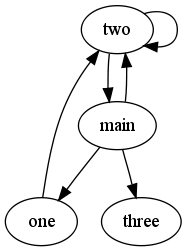
\includegraphics[scale=0.5]{img/normaln.png}
\else
	\includegraphics{img/normaln.ps}
\fi
\end{center}
\caption{Ukázka grafu volání}
\label{normaln-img}
\end{figure}

Z ukázkového grafu volání lze například vyčíst, že funkce \texttt{two} volá funkci \texttt{main} nebo že funkce \texttt{three} žádnou funkci nevolá. Pro zdrojový kód programu reprezentovaného grafem viz. výpis \ref{normal-c}.

\subsection{Implementace}
V nástroji je obsažen modul na generování grafu volání a jeho grafického znázornění. Pro tvorbu multigrafu a operace s ním jsem použil knihovnu \textsc{JGraphT}\cite{jgrapht}. Jedná se o velmi dobře dokumentovanou knihovnu pro práci s grafy v Javě. Knihovna je vydávána pod licencí \textsc{GNU LGPL}\footnote{GNU Lesser general public license. Kompletní znění na \url{http://www.gnu.org/copyleft/lgpl.html}.}. Graf je generován z XML reprezentace abstraktního syntaktického stromu. 

Pro vykreslení grafu je použit progam \textsc{Graphviz}\cite{graphviz}. Program je vydáván pod licencí CPL\footnote{CPL = Common Public License, celé znění na \url{http://www.graphviz.org/License.php}.}. \textsc{Graphviz} používá vlastní jazyk pro popis grafů který se nazývá \textsc{DOT}. Jazyk má jednoduchou gramatiku\footnote{Popis gramatiky jazyka \textsc{DOT}: \url{http://www.graphviz.org/doc/info/lang.html}} a je dobře zdokumentován. Pro použití programu \textsc{Graphviz} v Javě používáme obalovou třídu \texttt{cz.muni.fi.iti.scv.scvgui.GraphViz}.

Nástroj vygeneruje zdrojový kód jazyka \textsc{DOT} a ten buď zobrazí v GUI nebo při volání z CLI uloží obrázek ve formátu \textsc{PNG} do uživatelem zadaného souboru.

\begin{figure}[ht]
\begin{center}
\ifpdf
	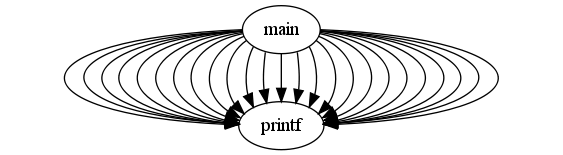
\includegraphics[scale=0.5]{img/many.png}
\else
	\includegraphics{img/many.ps}
\fi
\end{center}
\caption{Graf volání s mnoha voláními}
\label{many-img}
\end{figure}

\begin{lstlisting}[language=C,caption=Funkce s mnoha voláními,label=many-c]
int main() {
printf("call");
...
...
printf("call");
printf("call");

return 0;
}
\end{lstlisting}

\subsection{Graf bez vícenásobných hran}
Kromě grafu volání reprezentovaného multigrafem umí nástroj generovat i graf volání bez vícenásobných hran. Graf volání reprezentovaný multigrafem může být totiž už na celkem jednoduchých programech nepřehledný (viz. obrázek \ref{many-img}). Graf bez vícenásobných hran splňuje účel -- zobrazuje \uv{kdo koho volá}. Tento způsob generování grafu volání je v nástroji výchozí.

\subsection{Uživatelské rozhraní}
Modul je zakomponován jak v GUI nástroje, tak v CLI rozhraní. V GUI lze graf volání otevřených zdrojových textů zobrazit pomocí nabídky \textbf{Callgraph $\rightarrow$ Show Callgraph} nebo \textbf{Callgraph $\rightarrow$ Show Callgraph (single document)} pro graf volání aktuálně vybraného zdrojového textu. Třetí volba v nabídce (\textbf{Show strongly connected components}) slouží k zobrazení grafu volání s vyznačenými silně souvislými komponentami.

\begin{figure}[ht]
\begin{center}
\ifpdf
	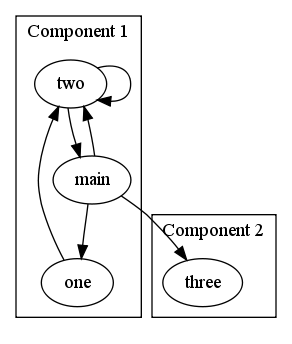
\includegraphics[scale=0.5]{img/normal.png}
\else
	\includegraphics{img/normal.ps}
\fi
\end{center}
\caption{Graf volání se zvýrazněnými silně souvislými komponentami}
\label{normal-img}
\end{figure}

Z příkazové řádky je graf volání generován pomocí volby \verb|--callgraph|. Pokud chceme, aby ve výstupu byly zvýrazněny silně souvislé komponenty, přidáme parametr \verb|--scc|. Pro generování grafu jako multigrafu je potřeba přidat volbu \verb|--cgm|.

\subsection{Volání funkce ukazatelem}
Při tvorbě grafu volání se nevyhodnocují žádné výrazy. Jedná se o reprezentaci statického modelu. 
Na obrázku \ref{pointer-img} je zobrazen graf volání programu, který používá volání pomocí ukazatele na funkci. Ukazatel není vyhodnocován a tudíž je v grafu zobrazeno volání \uv{funkce} \texttt{(*new\_function)}.


\begin{figure}[h]
\begin{center}
\ifpdf
	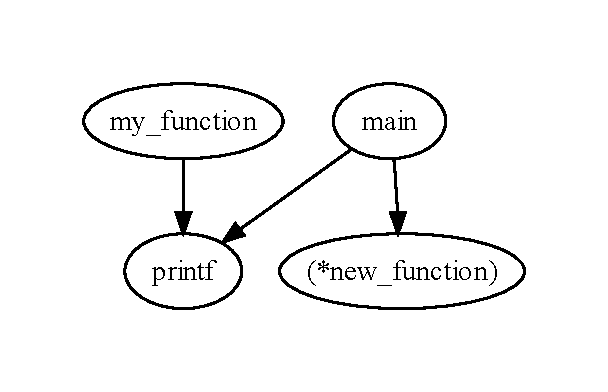
\includegraphics[scale=0.75]{img/pointer.pdf}
\else
	\includegraphics{img/pointer.ps}
\fi
\end{center}
\caption{Graf volání s ukazatelem}
\label{pointer-img}
\end{figure}

\begin{figure}[ht]
\begin{lstlisting}[language=C,caption=Funkce volaná ukazatelem,label=pointer-c]
static int my_function(int a)
{
    printf("my_function: %d\n", a);
    return (2*a + 3);
}

int main(void)
{
    int (*new_function)(int) = my_function;
    int  x;

    x = (*new_function)(10);
    printf("main: %d\n", x);
    return 0;
}
\end{lstlisting}
\end{figure}


\begin{figure}[ht]
\begin{lstlisting}[language=C,caption=Zdrojový kód použitý v ukázkách grafu volání,label=normal-c]
int main() {
        one();
        two();
        three();
}
int one() {
        two();
}
two() {
        main();
        two();
}
\end{lstlisting}
\end{figure}


%% =================================================================
%%				Static checker
%% =================================================================

\chapter{Nový static checker}\label{automaton-checker}

Tato kapitola popisuje práci na novém static checkeru. Hlavní nevýhodou řešení Jaroslava Novotného byl složitý zápis definičních souborů. Zápis se zaobíral zbytečnými implementačními detaily a spíš než aby popisovat automat, popisoval jeho implementaci. Moje řešení přináší mj. nový formát definičních souborů, jehož jednoduchost spočívá v tom, že se jedná o intuitivní zápis konečného automatu. S novým formátem definičních souborů bylo nutné naimplementovat znova i celou analýzu.

Nový checker nabízí uživateli také mnohem větší výrazovou sílu. Fragmenty kódu zde nejsou hledány jako konkrétní kusy XML zápisu AST, ani nejsou hledány pomocí \textsc{XPath} dotazů. Checker nabízí uživateli možnost jednoduše naimplementovat vlastní funkce, které budou fragmenty vyhledávat.

\section{Univerzální statický checker}
V současnosti je v nástroji implementován \textit{univerzální statický checker} jehož autorem je Jaroslav Novotný\cite{jarek}.

V této kapitole jsou zmiňovány celkem tři verze statického checkeru.
\begin{itemize}
	\item \textbf{Static checker old} je označení pro verzi z května 2007. Tato verze je detailně popsána v diplomové práci Jaroslava Novotného\cite{jarek}.
	\item \textbf{Static checker new} je označení pro verzi ze září 2007. Jedná o vylepšení verze z května téhož roku. Změny jsou popsány v sekci \ref{old-new}
	\item \textbf{Automaton checker} je kompletně přepracovaná verze, která je detailně popsána dále v této kapitole.
\end{itemize}

Jak původní dvě verze, tak i nejnovější verze, používají pro zápis automatu vyhledávajícího chyby \textit{XML definiční soubor}. Jedná se o soubor, který je checkeru předán na vstup společně se zdrojovými kódy, které má checker kontrolovat. Uživatel nástroje v tomto souboru definuje, jaké chyby chce hledat. První dvě verze mají podobný zápis. O změnách mezi těmito dvěma verzemi je hovořeno v následující sekci. Nejnovější verze (\textit{automaton checker}), kterou jsem implementoval v rámci této práce, používá zcela nový formát definičních souborů.

Výpis \ref{example-newchecker} a \ref{example-oldchecker} jsou ukázkou popisu automatu starší a novější verze starého přístupu \textit{static checker old} a \textit{static checker new}. Ve výpisu \ref{example-automatonchecker} je ukázán zápis definičního souboru \textit{automaton-checker}. Všechny popisují automat, který hledá stejný typ chyb -- ověřuje správnost zamykání.

\subsection{Změny ve \textit{static checker old}}\label{old-new}

Původní verze (\textit{static checker old}), která je detailně popsána v diplomové práci Jaroslava Novotného\cite{jarek}, byla během letní stáže ve firmě ANF DATA spol.~s~r.~o. modifikována a vznikla verze \textit{static checker new}. Byl kompletně změněn způsob vyhledávání fragmentů AST. V původní verzi bylo nutné do definičního souboru přímo vpisovat hledaný fragment tak, jak je reprezentován v XML AST. V nové verzi (\textit{static checker new}) je pro vyhledávání fragmentu použit výraz jazyka \textsc{XPath}\cite{xpath}. To dovoluje používat obecně silnější dotazy.

Verze \textit{static checker old} \uv{naplňuje} proměnné mechanismem známým z regulárních výrazů. Např. \texttt{(.*)unlock} do proměnné uloží všechny předpony slova \textit{unlock}. Stejné přiřazení se ve verzi \textit{static checker new} popíše pomocí elementu \texttt{get}, konkrétně \lstinline{<get>substring-before(./id[1]/text(), "unlock")</get>}.
 
V níže uvedených ukázkách (\ref{puvodni-findxml} a \ref{novy-findxml}) je demonstrován původní zápis deklarace proměnné a nový zápis deklarace stejné proměnné. V tagu \texttt{find} je uzavřen \textsc{XPath} výraz, podle kterého se hledají příslušné uzly v AST. Na každém nalezeném uzlu se potom spustí \textsc{XPath} dotazy \texttt{get}, jejichž návratové hodnoty se uloží jako hodnoty proměnné. Na hodnoty lze potom odkazovat pomocí jména zadaného v tagu \texttt{name}. Deklarace proměnné může obecně obsahovat více \texttt{get} výrazů. Celý odkaz na proměnnou se jménem \textit{LOCK} a výraz nalezený prvním \texttt{get} bude potom zapsán jako \verb|${LOCK:0}|.


\begin{lstlisting}[language=XML,caption=Zápis hledaného fragmentu v \textit{static checker old},label=puvodni-findxml]
    <var>
        <name>LOCK</name>
        <source>
            <functionCall>
                <id var="text">^(.*)unlock(.*)$</id>
            </functionCall>
        </source>
    </var>
\end{lstlisting}


\begin{lstlisting}[language=XML,caption=Zápis hledaného fragmentu v \textit{static checker new},label=novy-findxml]
    <var>
         <name>LOCK</name>
         <find>//functionCall[contains(./id[1]/text(), "unlock")]</find>
         <get>substring-before(./id[1]/text(), "unlock")</get>
         <get>substring-after(./id[1]/text(), "unlock")</get>
    </var>
\end{lstlisting}

V obou verzích platí, že když existuje více různých přiřazení do proměnné, provede se analýza pro každé přiřazení zvlášť. 


%% =================================================================
%%				Motivace
%% =================================================================
\section{Motivace ke změně}

Jak původní verze univerzálního statického kontroloru, tak pozměněná verze používá XML definiční soubory, které jsou pro člověka, který se systémem nepracoval, obtížné na porozumění. 

Definiční soubory původních verzí zacházely do zbytečných implementačních detailů. Uživatel nástroje, který neznal implementaci proto určité části definičního souboru nemohl pochopit.

Z tohoto důvodu vznikla potřeba přebudovat podobu XML definičních souborů do podoby, které velmi rychle porozumí i člověk, který se systémem ještě nepracoval.

Definiční soubor původní verze je navržen tak, že implementace analýzy byla celkem jednoduchou záležitostí. \textit{Automaton checker} byl navrhován obráceně. Nejprve byl navržena formát XML definičního souboru a až podle něj byl vytvářen algoritmus pro analýzu. Uživatel tak nemusí popisovat implementaci automatu, tak jako tomu bylo dříve. O implementaci se v \textit{automaton checkeru} stará nástroj, uživatel není implementačními detaily zatěžován.

Každý statický kontrolor je konečným automatem\cite{aag}. Snahou tedy bylo, aby XML definiční soubor byl co nejintuitivnějším zápisem konečného automatu.

V předchozí verzi se proměnné hledaly a přiřazovaly ještě před začátkem analýzy. Analýza se potom v cyklu opakovala pro každé přiřazení. To může být výkonnostním problémem. V \textit{automaton checkeru} se přiřazení hledají až za běhu a na jejich základě podle potřeby vznikají dynamicky nové automaty.

Nový přístup je obecnějším popisem automatu, uživateli nabízí širší výrazovou sílu. Ve verzi \textit{static checker old} bylo při vyhledávání určitého fragmentu kódu vpisovat přímo kus XML kódu AST. Tento přístup byl sice změněn (popis změn viz. \ref{old-new}) a v novější verzi lze vyhledávat fragmenty pomocí výrazů \textsc{XPath}. \textit{Automaton checker} nabízí mnohem silnější způsob hledání fragmentů kódu. Funkci pro vyhledávání fragmentu si může uživatel zadefinovat sám. Vyhledávání fragmentu kódu je v této kapitole popisováno jako \uv{podmínka pro přechod}. V sekci \ref{interface-trigger} je popsáno, jak vytvořit uživatelskou funkci pro vyhledávání.

Cílem nového checkeru je i snadnější rozšiřitelnost. Kromě možnosti zadefinovat funkci pro vyhledávání je uživateli je nabízena možnost použít typy proměnných, které si sám nadefinuje. V sekci \ref{interface-param} je popsáno, jak lze novou proměnnou zadefinovat.


%% =================================================================
%%				Popis XML
%% =================================================================

\section{Popis XML definičního souboru}

V této sekci je popsán formát XML dokumentu, který je společně s testovaným zdrojovým checkeru. XML je popisem konečného automatu, který je spuštěn na zdrojovém kódu při analýze. Ukázka takového dokumentu je ve výpisu \ref{example-automatonchecker}.


Kořenový tag dokumentu se jmenuje {\tt automaton}. Aby soubor splňoval požadavky správně strukturovaného XML dokumentu, musí být v dokumentu tento element obsažen právě jednou a obklopuje všechny ostatní elementy dokumentu.

\begin{lstlisting}[language=XML]
<automaton>
	<!-- Metadata -->
	<!-- Proměnné -->
	<!-- Stavy a přechody -->
</automaton>
\end{lstlisting}


\subsection{Metadata}
Pro přehlednost lze automatu pomocí tagů {\tt name} a {\tt description} zadat jméno a textový popisek. Hodnoty těchto tagů nemají žádný vliv na funkci automatu (zejména se podle nich neřídí unikátnost automatu). Slouží k jednodušší identifikaci automatu například v reportech.

\begin{lstlisting}[language=XML]
<automaton>
  <name>Locking checker</name>
  <description>Checks locks with one argument as the name of the lock</description>
...
</automaton>
\end{lstlisting}

\subsection{Proměnné}\label{params}
Automat je možné parametrizovat pomocí proměnných. Každá proměnná automatu má svůj, v rámci automatu unikátní identifikátor a svůj typ.

Jedná se o obdobu deklarace proměnné známé z většiny moderních programovacích jazyků. Identifikátor je zadán hodnotou elementu {\tt id}. Tímto identifikátorem se lze na proměnnou odkazovat v dalších částech definičního souboru. Z toho vyplývá i zmíněný požadavek na unikátnost.

Typ proměnné je definován hodnotou elementu {\tt class}. Jedná se o kompletní název třídy, která reprezentuje tento typ proměnné. Tato třída musí implementovat rozhraní {\tt AutomatonParam}. Více o implementaci tohoto rozhraní viz. \ref{toc-interface}.

\begin{lstlisting}[language=XML]
<automaton>
...
<param>
        <id>x</id><!--  Unikatni identifikator parametru. -->
        <class>cz.muni.fi.iti.scv.newchecker.AutomatonParamParamNames</class><!-- Udava typ parametru -->
  </param>
...
</automaton>
\end{lstlisting}


Implementace proměnných a jejich typů vychází z tzv. \emph{hole variables} a jejich typů \emph{hole types} používaných v jazyce \textsc{Metal}. Popis tohoto přístupu se nachází v \cite{engler-pldi} a \cite{engler-paste}. Checkery psané v jazyce Metal jsou spouštěny jako rozšíření překladače. Pro překlad se používá upravená verze překladače \textsc{gcc} -- překladač \textsc{xgcc}. To umožňuje v jazyce \textsc{Metal} používat běžné typy jazyka C jako např. {\tt int, double, float,} \ldots.

% =================================================================
% 			AUTOMAT
% =================================================================
\newpage
\paragraph{Definice}\cite{aag} Formálně je \emph{konečný automat} definován jako uspořádaná pětice $(Q, \Sigma, \sigma, q_0, F)$, kde:
\begin{itemize}
	\item $Q$ je neprázdná množina \emph{stavů}.
	\item $\Sigma$ je množina vstupních symbolů, nazývaná také \emph{vstupní abeceda}.
	\item $\sigma: Q \times \Sigma \rightarrow Q$ je parciální \emph{přechodová funkce}.  
    \item $q_0 \in Q$ je \emph{počáteční stav}.
	\item $F \subseteq Q$ je množina \emph{koncových stavů}. 
\end{itemize}

\subsection{Konečný automat}

\begin{lstlisting}[language=XML,caption=Zápis stavu konečného automatu]
<state initial="true">
    <name>U</name> <!-- V ramci automatu unikatni -->
    <description>Unlocked</description>
    <transition> <!-- Kazdy state ma alespon jeden transition. Finalni stavy totiz za stavy nepovazujeme (neevidujeme je) -->
            <trigger>
                    <pass>lock</pass> <!-- Predava se jako parametr metode loadTrigger  -->
                    <class>cz.muni.fi.iti.scv.newchecker.FunctionNameTrigger</class>
                    <param>x</param>
            </trigger><!-- Akce, pod kterou se prejde do <to> stavu-->
            <to>L</to><!-- Name stavu, do ktereho se prejde -->
    </transition>

    <transition>
            <trigger>
                    <pass>unlock</pass>
                    <class>cz.muni.fi.iti.scv.newchecker.FunctionNameTrigger</class>
                    <param>x</param><!-- Zde se odkazujeme na parametry. Na poradi zalezi. -->
            </trigger>
            <errmsg>Double unlock!!</errmsg><!-- Misto "to" muze byt errmsg. To znamena, ze se dostavame do chyboveho stavu. Automat konci -->
    </transition>

</state>
\end{lstlisting}

Výše uvedené položky jsou v XML dokumentu popsány těmito elementy:
\begin{itemize}
	\item $Q$ (množina \emph{stavů}) je množina elementů {\tt state}. Pro splnění definice kromě těchto, explicitně definovaných, stavů existuje ještě \emph{virtuální chybový stav} (viz. \ref{virtual-state}). Ten se do dokumentu nezapisuje.
	
	\item $\Sigma$ (množina vstupních symbolů) není v dokumentu explicitně definována. Vstupní symbol je definován u přechodové funkce (elementem {\tt trigger}).
	
	\item $\sigma: Q \times \Sigma \rightarrow Q$ (parciální přechodová funkce) je definována elementy {\tt transition}. Automat na každé hraně CFG může a nemusí přejít do jiného stavu. Vstupní slovo je tedy definováno jako hrany CFG, které jsou pro automat z hlediska analýzy zajímavé.
		
    \item $q_0 \in Q$ (\emph{počáteční stav}) je element {\tt state}, který má argument {\tt initial} nastaven na hodnotu {\tt true}. Podle definice se takový element v dokumentu musí nacházet právě jednou. Nástroj tuto podmínku kontroluje.
  
	\item $F \subseteq Q$ (\emph{koncových stavů}) je definována jako množina stavů (element {\tt state}), které neobsahují element {\tt eor}.
	 
\end{itemize}

\begin{figure}[ht]
\begin{center}
\ifpdf
	\includegraphics[width=6cm]{img/automaton.png}
\fi
\end{center}
\caption{Konečný automat pro analýzu zámků}
\label{lock-automaton}
\end{figure}


% \paragraph{Virtuální stav}
\label{virtual-state}Automat může obsahovat jeden \emph{virtuální chybový stav}. V ukázce \ref{lock-automaton} je to stav označený V. To je stav, ze kterého neexistuje žádný přechod. Pokud se automat dostane do tohoto stavu, značí to nalezenou chybu v analýze. Přechod ({\tt transition}) směřující do tohoto stavu musí vždy obsahovat chybové hlášení {\tt errmsg}. V obrázku \ref{lock-automaton} je hlášení uvozeno heslem \uv{Err}. Chybové hlášení v XML definičním souboru nahrazuje cílový uzel {\tt to}.

Akceptování automatem při analýze znamená, že při analýze nebyla nalezena chyba. 

\subsection{Zápis automatu}

\paragraph[state]{\texttt{state} -- stavy}
Každý element \texttt{state} musí obsahovat element {\tt name}. Jeho hodnota je unikátním ukazatelem tohoto stavu a slouží k odkazování na něj (například v přechodové funkci).

Dalším povinným elementem elementu \texttt{state} je \texttt{description}. Jeho hodnota se používá v uživatelských výpisech a měla by jednoznačně a jasně určovat stav, který popisuje (např. pro testování správného zamykání by ideální \texttt{description} pro stav, kdy je zámek zamčen, byla ideální hodnota \emph{Locked}).

\begin{lstlisting}[language=XML,caption=Zápis elementů \texttt{state}{,} \texttt{name} a \texttt{description}]
<state initial="true">
    <name>U</name> <!-- V ramci automatu unikatni -->
    <description>Unlocked</description>
    ...
</state>
\end{lstlisting}

\paragraph[transition]{\texttt{transition} -- přechody}
Každý stav \texttt{state} potom musí obsahovat alespoň jeden přechod \texttt{transition}. 
% Stav, ze kterého nelze přejít do žádného jiného stavu je \hyperref[virtuální stav]{virtual-state}, který se do XML zápisu nezapisuje.


\begin{lstlisting}[language=XML,caption=Zápis elementů \texttt{transition}]
<state initial="true">
    ...
	<transition>...</transition>
    <transition>...</transition>
	...
</state>
\end{lstlisting}

\paragraph[trigger]{\texttt{trigger} -- podmínka přechodu}
Každá \texttt{transition} musí obsahovat právě jeden \texttt{trigger}. Ten určuje podmínku, pod kterou se přejde do jiného stavu, případně pod kterou se vypíše chyba.


Element \texttt{trigger} musí vždy obsahovat element \texttt{pass}. Jeho obsah je předán jako parametr metodě \texttt{loadTrigger} (viz. \ref{toc-interface}). Druhým povinným elementem je \texttt{class}. Hodnota tohoto parametru je názvem třídy, která bude instanciována a použita pro tento trigger. Následovat může nula a více elementů \texttt{param}. Tyto parametry se odkazují na parametry deklarované na začátku dokumentu (viz. \ref{params}).

\begin{lstlisting}[language=XML,caption=Zápis \texttt{trigger}]
<trigger>
        <pass>unlock</pass>
        <class>cz.muni.fi.iti.scv.newchecker.FunctionNameTrigger</class>
        <param>x</param><!-- Zde se odkazujeme na parametry. Na poradi zalezi. -->
</trigger>
\end{lstlisting}


\paragraph[to a errmsg]{\texttt{to} a \texttt{errmsg}}
Každý element \texttt{transition} musí obsahovat právě jeden element \texttt{to} nebo \texttt{errmsg}. Pokud je splněna podmínka pro \texttt{trigger} daného \texttt{transition} a je obsažen element \texttt{to}, automat přejde do stavu definovaného hodnotou tohoto elementu. Pokud je místo \texttt{to} obsažen \texttt{errmsg} a je splněna podmínka pro přechod, je při analýze hlášena chyba. V tomto případě přechází automat do zmiňovaného virtuálního chybového stavu a na analýze se dále nepodílí.
\begin{lstlisting}[language=XML,caption=Zápis \texttt{to}]
<to>L</to><!-- Misto "to" muze byt errmsg. To znamena, ze se dostavame do chyboveho stavu. Automat konci -->
\end{lstlisting}


%% =================================================================
%%				Rozhrani
%% =================================================================

\section{Rozhraní}\label{toc-interface}
Za účelem rozšiřitelnosti je možné pro některé části analýzy používat vlastní implementaci některých rozhraní. 
Konkrétně se jedná o možnost implementace vlastního typu parametru (proměnné) a triggeru -- pro trigger existuje v nástroji rozhraní {\tt TransitionTrigger} a pro parametr rozhraní {\tt AutomatonParam}. Na implementace těchto rozhraní se lze odkazovat v XML definičním souboru. Pro trigger hodnotou elementu {\tt class} v elementu {\tt trigger}, v případě parametru potom hodnotou elementu {\tt class} v elementu {\tt param}. Dodržení implementace daných rozhraní je při načítání XML definičního souboru kontrolováno.

Do nástroje je vše zakomponováno pomocí \textsc{Java Reflection API}. Nové objekty jsou zde instanciovány bez volání konstruktoru. Místo konstruktoru má každé rozhraní metodu, která je volána \uv{místo} konstruktoru. V rozhraní \texttt{TransitionTrigger} se jedná o metodu \texttt{loadTrigger} a v \texttt{AutomatoParam} o \texttt{setId}. Tyto metody jsou volány bezprostředně po instanciaci a slouží k inicializaci parametrů.

Kompletní popis rozhraní lze najít v \textsc{javadoc} dokumentaci, přiložené na CD.


\subsection[TransitionTrigger]{Rozhraní \texttt{TransitionTrigger}}\label{interface-trigger}

\begin{figure}[ht]
\begin{center}
\ifpdf
	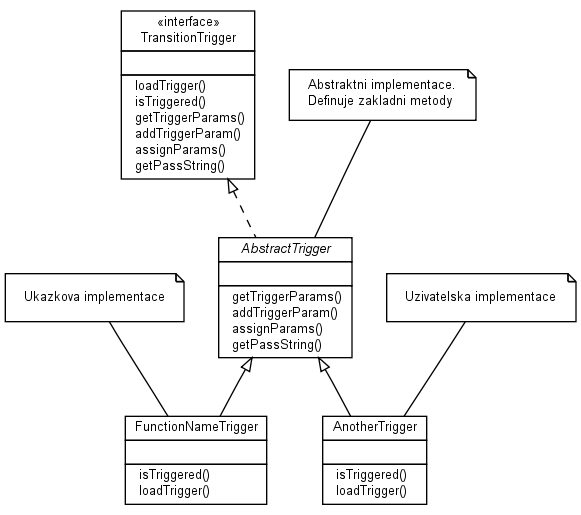
\includegraphics[width=12cm]{img/trigger.png}
\fi
\end{center}
\caption{Diagram tříd pro rozhraní TransitionTrigger}
\label{transition-trigger-classdiagram}
\end{figure}

Trigger (spouštěč) zjednodušeně slouží k nalezení zajímavé části AST. Implementace určuje, za jaké podmínky bude trigger spuštěn. K tomuto rozhraní existuje v nástroji abstraktní implementace, která má základní operace již naimplementovány. Vedle ní je v nástroji přítomna i ukázková implementace \texttt{cz.muni.fi.iti.scv.newchecker.FunctionNameTrigger}. Ta vyhledává uzly podle názvu volané funkce.

Rozhraní určuje tyto metody:

\paragraph{\texttt{void loadTrigger(String pass)}} je metoda \uv{nahrazující} konstruktor -- tato metoda je vždy volána hned po instanciaci třídy. Jako parametr dostává metoda obsah elementu {\tt pass} v elementu {\tt trigger}. Tato hodnota slouží k nastavení dané instance. Například v triggeru, který hledá uzly podle názvu volané funkce, by tímto parametrem byl název hledané funkce. Omezení na datový typ {\tt String} je dáno vazbou na XML. Pokud implementátor potřebuje triggeru předat více parametrů při inicializaci, může si tento řetězec například libovolně zpracovat.

\paragraph{\texttt{void addTriggerParam(AutomatonParam param)}} je metoda sloužící k přidání jednoho parametru k triggeru. Toto se děje při načítání XML definičního souboru. Tato metoda je volána pro každý parametr automatu znovu a na pořadí volání záleží. Každý parametr má totiž svoje pořadí. Této znalosti lze využít při inicializaci hodnoty parametru. Při načítání XML definičního souboru je metoda volána v pořadí zápisu elementů. 

Na pořadí přidávání parametrů do triggeru záleží a při načítání XML definičního souboru je tato metoda volána pro každý element {\tt param} v pořadí, ve kterém jsou parametry uvedeny. 

\paragraph{\texttt{List<AutomatonParam> getTriggerParams()}} vrací seznam parametrů triggeru v pořadí, ve kterém byly do triggeru přidány.

\paragraph{\texttt{Set<AssignedParam> assignParams(CFGNode from, CFGNode to)}} slouží k přiřazení hodnot parametrům. Abstraktní implementace toto volání předává metodě \texttt{initValue} třídy \texttt{AutomatonParam}. Návratovou hodnotou je množina instancí třídy \texttt{AssignedParam}, ve které každý prvek odpovídá jednomu přiřazenému parametru.

\paragraph{\texttt{boolean isTriggered(CFGNode from, CFGNode to)}} je klíčovou metodou tohoto rozhraní. Při analýze je aktuálním instancím triggerů nabídnuta dvojice uzlů CFG. Pokud je pro danou dvojici splněna podmínka pro přechod, vrací metoda {\tt true}, jinak vrací {\tt false}.  

\paragraph{\texttt{String getPassString()}} vrací řetězec předávaný jako parametr metodě {\tt loadTrigger(String pass)}. 


\subsection[AutomatonParam]{Rozhraní \texttt{AutomatonParam}}\label{interface-param}

\begin{figure}[ht]
\begin{center}
\ifpdf
	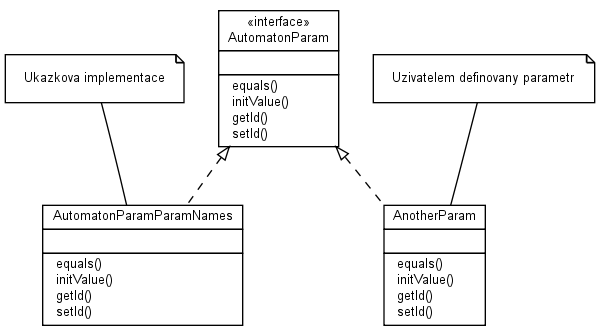
\includegraphics[width=12cm]{img/param.png}
\fi
\end{center}
\caption{Diagram tříd pro rozhraní AutomatonParam}
\label{param-classdiagram}
\end{figure}

Toto rozhraní musí implementovat všechny třídy, které chceme používat jako parametry automatu. Lze je přirovnat k typům proměnných používaných v typovaných jazycích. Nástroj nabízí uživateli zadefinovat si svůj vlastní typ. Ukázkovou implementací je třída {\tt AutomatonParamParamNames}, která reprezentuje jména argumentů volání funkce.

\paragraph{\texttt{void setId(String id)}} nastavuje unikátní identifikátor parametru. Pomocí tohoto identifikátoru je na parametr odkazováno. Tato metoda je \uv{náhradou} konstruktoru -- nastavuje parametry.

\paragraph{\texttt{String getId()}} vrací hodnotu unikátního identifikátoru. 

\paragraph{\texttt{AssignedParam initValue(CFGNode from, CFGNode to, int index)}} \emph{inicializuje} hodnotu proměnné. Tato metoda nemění stav objektu, výsledek volání je vrácen v podobě instance třídy {\tt AssignedParam}. K nastavení hodnoty může metoda použít zdrojový a cílový uzel v CFG (ze kterých lze například získat AST) a pořadí parametru ({\tt index}). Pořadí je v ukázkové implementaci (argumenty volané funkce) použito v \textsc{XPath} dotazu, který vyhledává jednotlivé argumenty. Všechny parametry jsou totiž instanciovány na jedné hraně CFG (hodnota {\tt from} a {\tt to}) je u všech volání stejná.

\paragraph{\texttt{boolean equals(Object other)}} je metoda, kterou je vhodné překrýt. Tato metoda je definována ve třídě {\tt Object}. Ideální implementací je porovnání unikátních ukazatelů obou instancí (společně s dalšími povinnými náležitostmi metody equals). Pokud se přetěžuje metoda {\tt equals}, měla by být přetížena i metoda {\tt hashCode}\cite{java-efektivne}.
   

%% =================================================================
%%				ALGORITMUS
%% =================================================================

\section{Algoritmus analýzy}
Hlavní algoritmus nového checkeru je obsažen ve třídě {\tt Automaton}. Ta obsahuje mimo jiné i statickou metodu {\tt main}, které je zavolána při spuštění binárního souboru. Při spuštění z příkazové řádky jsou přijímány dva argumenty -- první určuje cestu k souboru se zdrojovým kódem, který má být analyzován a druhý určuje cestu k XML definičnímu souboru.

Třída neobsahuje veřejný konstruktor. K instanciaci třídy slouží statický tovární metoda \lstinline[language=Java]{getInstanceByDocument(Document doc)}. Jako argument přijímá XML definiční soubor. Metoda ověří jeho nejdůležitější náležitosti (jedinečnost počátečního stavu apod.) a vrátí nový, popisu odpovídající automat.

Poté, co se do automatu načte metodou {\tt loadDocument(Document source)} AST programu, který má být analyzován, lze zavolat metodu {\tt run()}, která spustí vlastní analýzu.

\subsection{Pomocné třídy}

\paragraph{\texttt{AssignedParam}}
je jednoduchá třída, která reprezentuje přiřazení hodnoty parametru. Hodnota je reprezentována typem \texttt{String}.

\paragraph{\texttt{RunningAutomaton}}
Instance třídy {\tt RunningAutomaton} popisuje běžící automat. Zatímco třída \texttt{Automaton} je popisem automatu (stavy, přechody, \ldots), instance této třídy je popisem jednoho konkrétního běhu. Běžící automat má již inicializované hodnoty svých parametrů (množina instancí třídy \texttt{AssignedParam}) a drží si informaci o stavu, ve kterém se právě nachází (\texttt{currentState}). Běžící automat je jednoznačně identifikován atributem \texttt{id}. Jedná se o celé číslo, které je mu přiřazeno při instanciaci. Kromě tohoto identifikátoru si instance drží i množinu identifikátorů všech svých předchůdců. V této množině je vždy obsaženo vlastní ID a v případě, že je automat vytvořen jako kopie jiného automatu, je obsažena i množina ID předchůdců.

Metoda \texttt{RunningAutomaton getCopy()} vrací kopii běžícího automatu. Nově vytvořený automat dědí vše kromě ID. Do množiny ID nově vytvořeného automatu je automaticky vložena množina ID předchůdce.

\paragraph{\texttt{RunningAutomataSet}}
Instance třídy \texttt{RunningAutomataSet} je množinou objektů \texttt{RunningAutomaton}. Kromě standardních množinových operací obsahuje pomocnou metodu \texttt{RunningAutomataSet getCopy()}\label{set-get-copy}, která vrátí množinu kopií automatů obsažených v množině.

\paragraph{\texttt{Pair}}
reprezentuje uspořádanou dvojici. Je použit mechanizmus generics jazyka Java díky němuž je zajištěna typová kontrola. Třída neobsahuje veřejný konstruktor, ale pouze statickou tovární metodu \texttt{getInstance}. Do té lze v budoucnu naimplementovat např. cache.

\paragraph{\texttt{AutomatonState}} 
popisuje stav automatu. Stav je jednoznačně identifikován svým ID. Obsahuje odkaz na všechny přechody, které s něj vycházejí a metodu \texttt{getTransitionByTriggeredTrigger}, která přijímá jako argument hranu CFG a pokud existuje nějaký přechod, jehož trigger je pro danou hranu \uv{spuštěn}, je tento přechod vrácen, jinak je vráceno \texttt{null}.

\paragraph{\texttt{AutomatonTransition}} popisuje přechod automatu z jednoho stavu do jiného stavu. Metoda \texttt{isError()} vrací informaci o tom, zda přechod vede do virtuálního chybového stavu.  V případě že vrací \texttt{true}, vrací metoda \texttt{getErrorMessage()} chybové hlášení. 

Pokud metoda \texttt{isEOR()} vrací \texttt{true}, značí to, že v uzlu, ve kterém je přechod obsažen, nesmí analýza skončit. Pokud zde skončí, značí to chybu.

\paragraph{\texttt{EdgeWithAutomata}}
je třída popisující hranu s automaty. Tato obálka se používá v zásobníku hran, které mají být ještě projity. Kromě getterů a setterů obsahuje třída metodu \texttt{deleteDuplicateAutomata(\\ Set<Pair<Integer, Integer>> pairs)}. Tato metoda na základě argumentu promaže všechny \uv{duplicitní} automaty. Argumentem je množina uspořádaných dvojic ceých čísel, kde první prvek označuje ID automatu a druhý označuje ID stavu. Automat je pro danou hranu považován za duplicitní, pokud na této hraně již byl spuštěn automat, který je jeho předchůdcem a na dané hraně byl ve stejném stavu.

\paragraph{\texttt{EdgeStack}} 
popisuje zásobník\footnote{Zásobník je datová struktura typu LIFO (Last In First Out)}. Má přetíženou metodu \texttt{push} tak, že je zajištěno, že na zásobníku nebudou duplicitní hrany. Pokud je vkládána hrana, která na zásobníku již je, tak se místo přidávání nové hrany s automaty k původní hraně přidají automaty, které měly být přidány s přidávanou hranou. Automaty přiřazené k hraně jsou reprezentovány množinou, tudíž je zajištěno, že stejný automat nebude na hraně spuštěn vícekrát.

% ===================================================
% 			RUN
% ===================================================
\subsection{Metoda \texttt{run()}}
Samotná analýza používá graf toku řízení jednotlivých funkcí. Ve zdrojovém AST se tedy najdou všechny definice funkce (uzly \texttt{functionDefinition}) a z každého se pomocí modulu \texttt{xml2cfg}, vygeneruje potřebný graf toku řízení. Analýza se potom spouští pro každou funkci zvlášť.

Hlavní algoritmus pro svůj běh používá tyto paměti:
\begin{itemize}
	\item \textbf{edgeStack} je zásobník, na který se ukládají hrany, které je potřeba ještě projít a automaty, které se mají na příslušných hranách spustit. Zásobník je reprezentován objektem \texttt{EdgeStack}
	\item \textbf{edgeHistory} je datová struktura, ve které se ukládá historie již projitých hran a dvojic automat---stav, které se na dané hraně spouštěly. Za účelem paměťové efektivity se ukládají pouze ID automatů a ID stavů. Jedná se o mapu, kde klíčem je ID hrany. Každá hrana může tedy být v mapě obsažena maximálně jednou.
\end{itemize}

Na začátku analýzy se na zásobník \textbf{edgeStack} přidají všechny hrany, které vycházejí z počátečního uzlu CFG (ten je podle definice\cite{jarek} vždy právě jeden).

Následuje \textit{while--do} cyklus, který jako podmínku testuje neprázdnost zásobníku \textbf{edgeStack}. Na začátku každého průchodu se odebere prvek z vrcholu zásobníku (operace \texttt{pop()}) a ten je tělem cyklu zpracován.

\subsubsection{Změna stavu automatu}
Nejdříve se analýza snaží najít a pohnout některým z již běžících automatů aktuální hrany. Všem automatům právě zpracovávané hrany je hrana nabídnuta. Pokud některý automat vrátí pro tuto hranu transition (podmínka pro trigger je pro tuto hranu splněna), tak vyhledávání končí a stav automatu, který transition vrátil se podle ní mění. Pokud transition vede do virtuálního chybového stavu, vypíše se chyba a automat si tuto skutečnost poznamená (automat sice interně do žádného uzlu nepřejde, stejná chyba se ale vícekrát hlásit nebude).

Pokud se nepodaří hnout žádným běžícím automatem, nabídne analýza hranu k vytvoření nového běžícího automatu. Automat hledá pomocí metody \texttt{isTriggered} z rozhraní \texttt{TranistionTrigger} transition vedoucí z počátečního stavu. Pokud o hranu \uv{má zájem} a vrátí transition, vytvoří se nový běžící automat a jeho stav se nastaví podle nalezeného transition. Pokud transition vede do virtuálního chybového stavu, vypíše se opět chybové hlášení a nově vytvořený automat si tuto skutečnost poznamená. Nově vytvořený automat se přidá do množiny automatů pro aktuální hranu.

\subsubsection{Poslední hrana}
Pokud aktuální hrana vede do koncového bodu CFG, je nutné otestovat, jestli některý s automatů, vázaných na aktuální hranu, není ve stavu, ve kterém nesmí skončit. Třída \texttt{ControlFlowGraph} obsahuje metodu \texttt{getEndNode()}, která vrací koncový uzel grafu toku řízení. Informaci o tom, jestli je automat ve stavu, ve kterém nesmí skončit, poskytuje metoda \texttt{getEOR()} třídy \texttt{AutomatonState}.
 
Pro každý automat aktuální hrany, který je ve stavu, ve kterém nesmí skončit, vypíše chybu. 

\subsubsection{Historie}
V historii prošlých hran (\textbf{edgeHistory}) je každá hrana maximálně jednou. S každou hranou je v historii asociována množina uspořádaných dvojic ID automatu---ID stavu. Ukládání informací do historie musí předcházet operaci přidávání hran na zásobník, protože historii hran používáme k filtrování duplicit na zásobníku. V historii jsou vždy ukládány cílové stavy automatů na dané hraně. Tento přístup je vhodný při filtrování, protože na zásobník se ukládají hrany ke zpracování a u nich je výchozím stavem cílový stav tohoto průchodu.

\subsubsection{Přidání hran na zásobník}
Podle specifikace CFG může mít uzel žádného, jednoho nebo dva následníky. Žádného následníka má z definice\cite{jarek} právě tehdy když se jedná o koncový uzel. Dva následníky má uzel právě tehdy když se jedná o větvení (podmínka {\tt if-then-else}, {\tt while} cyklus, apod.). Konstrukt {\tt switch} je rozbit na posloupnost {\tt if-then-else} větvení. Ve všech ostatních případech má každý uzel právě jednoho následníka. Při přidávání na zásobník se sledují následníci koncového uzlu zpracovávané hrany.

Pokud nemá uzel žádné následníky, na zásobník se nic nepřidává.

Pokud má uzel právě jednoho následníka, přidá se na zásobník hrana, která vede do uzlu následníka, a množina všech automatů právě zpracovávané hrany. Tato množina již obsahuje i nově vytvořené automaty.

Pokud má uzel právě dva následníky, jsou na zásobník vloženy obě hrany. K jedné hraně je připojena množina referencí na automaty právě zpracovávané hrany. K druhé hraně je připojena množina kopií aktuálních automatů. Kopie množiny automatů se vytváří pomocí metody \texttt{getCopy()} (viz. \ref{set-get-copy}). Na zásobník je nejdříve vložena hrana s kopiemi a až potom hrana s referencemi na aktuální automaty. Zásobník je totiž strukturou LIFO z čehož vyplývá, že později přidaný prvek bude dříve odebrán a tím pádem i dříve zpracován. Z hlediska analýzy je výhodnější projít nejdříve hranu s \uv{originálními} automaty a až potom hranu s kopiemi. 

Po přidání každé hrany na zásobník se prořezávají k hranám připojené automaty a mažou se duplicity. Prořezává se na základě historie. Z množiny automatů na zásobníku se vymažou všechny takové automaty, které na dané hraně již byly spuštěny a jejich stav byl stejný, jako stav přidávaného automatu. Odstraněny jsou také ty, které mají předchůdce, který byl na dané hraně spuštěn se stejným stavem.

Zde končí zpracování jedné hrany a pokud je na zásobníku nějaká hrana ke zpracování, zpracuje se další hrana.


%% =================================================================
%%				ZÁVĚR
%% =================================================================

\chapter{Závěr}

Tato práce popisuje moduly, které jsem zakomponoval do již existujícího nástroje na statickou analýzu, vyvíjeného v laboratoři ITI na Fakultě informatiky. Popsány jsou jak obecné práce na nástroji (podpora argumentů příkazové řádky, logování pomocí nástroje \textsc{log4j} a modul pro generování grafu volání), tak i zcela nový statický checker -- \textit{automaton checker}.

\textit{Automaton checker} jsem vytvářel s cílem vyvinout checker, který bude ovládán XML definičními soubory, které jsou lehce čitelné i pro člověka, který s nástrojem nepracoval. Definiční soubory jsou jednoduchým popisem konečného automatu, což zajišťuje požadovanou jednoduchost a čitelnost. Formát těchto souborů práce detailně popisuje.

Na rozdíl od předchozích implementací univerzálního statického checkeru v nástroji nepopisují definiční soubory implementační detaily, ale popisují automat tak, jak je obecně znám (stavy, přechody, \ldots).

Velký důraz je kladen na rozšiřitelnost. \textit{Automaton checker} nabízí možnost definovat vlastní typy proměnných a vlastní funkce pro vyhledávání fragmentů kódu. V předchozích verzích se fragmenty hledaly buď přímým zápisem kusu XML AST nebo později \textsc{XPath} dotazem. Oba přístupy jsou v porovnání s novým řešením velmi slabé.

Pro lepší začlenění do nástroje bude potřeba sjednotit způsob hlášení chyb s ostatními komponentami (implementovat rozhraní \texttt{Checker}).

V \textit{automaton checkeru} bude potřeba vylepšit a zefektivnit také způsob promazávání duplicit v historii při analýze programu. Za účelem nízké paměťové náročnosti se v historii používají unikátní celočíselné identifikátory. Tento přístup umožňuje promazávat duplicity, které vznikly kopií již běžícího automatu, ale neposkytuje informaci o tom, jaké automaty byly na dané hraně nově vytvořeny. Při vícenásobném procházení stejné hrany se potom stane, že automat bude vytvořen při každém běhu znova.

Pro pohodlí uživatele nástroje bude také potřeba připravit více typů parametrů. Tato práce obsahuje pouze jednu referenční implementaci.


%% =================================================================
%%				Zdroje
%% =================================================================


\cleardoublepage
\bibliographystyle{czechiso}  % bibliografický styl 
\phantomsection
\addcontentsline{toc}{chapter}{Literatura}
\bibliography{latin-zdroje} % soubor s citovanými
                           % položkami bibliografie 



\appendix
\chapter{Obsah přiloženého CD}
\begin{description}
	\item[\texttt{/automaton-dist/}] Obsahuje binární distibuci nástroje ve formátu \textsc{jar}. V této distribuci je nastavena třída \texttt{Automaton} jako hlavní. \textit{Automaton checker} takze lze spouštět přímo z příkazové řádky pomocí\\ \texttt{java -jar automaton.jar <AnalyzovanyProgram>\\ <XMLDefinicniSoubor>}.
	\begin{description}
		\item[\texttt{/lib/}] obsahuje potřebné knihovny.
	\end{description}
	
	
	\item[\texttt{/automaton-checker/}] Ukázky XML definičních souborů \textit{automaton checkeru} a zdrojové kódy, na kterých lze analýzu vyzkoušet.
	
	\item[\texttt{/callgraph/}] Ukázky vygenerovaných grafů volání a zdrojových kódů, ze který jsou generované.
	
	\item[\texttt{/dist/}] V tomto adresáři je obsažena nástroj v binárním formátu \textsc{jar}.
	\begin{description}
		\item[\texttt{/lib/}] obsahuje knihovny, které nástroj využívá.
	\end{description}
	
	\item[\texttt{/thesis/}] obsahuje zdrojový text bakalářské práce i vygenerované \textsc{PDF}. Obsaženy jsou i všechny použité obrázky.
	
	\item[\texttt{/staticchecker-old/}] obsahuje ukázky starší verze statického checkeru (\textit{static checker old}) společně s ukázkovými zdrojovými kódy.
	
	\item[\texttt{/staticchecker-new/}] obsahuje ukázky novější verze statického checkeru (\textit{static checker new}) společně s ukázkovými zdrojovými kódy.
	
	\item[\texttt{/src/}] Kompletní zdrojové kódy nástroje v jazyce Java.
	
	\item[\texttt{/xsd/}] obsahuje popis schématu XML pro popis AST.	

\end{description}


\chapter{Ukázky XML definičních souborů}

\section{Verze \textit{static checker old}}

\begin{lstlisting}[language=XML,caption=Zápis definičního souboru pro \textit{static checker old},label=example-oldchecker]
<checker>
    <info>
        <name>Locking-checker</name>
        <description>Checks if the functions 'lock()' and 'unlock()' are correctly paired.</description>
    </info>

    <definition>
        <beginState>U</beginState>

        <propagationRule>
            <description>Locking.</description>
            <source>
                <functionCall>
                    <id>lock</id>
                </functionCall>
            </source>
            <stateAction>
                <set>L</set>
            </stateAction>
        </propagationRule>

        <propagationRule>
            <description>Unlocking.</description>
            <source>
                <functionCall>
                    <id>unlock</id>
                </functionCall>
            </source>
            <stateAction>
                <set>U</set>
            </stateAction>
        </propagationRule>

        <errorRule>
            <name>Double-lock</name>
            <description>Function is locking the lock that si already locked.</description>
            <state>
                <contains>L</contains>
            </state>
            <source>
                <functionCall>
                    <id>lock</id>
                </functionCall>
            </source>
        </errorRule>

        <errorRule>
            <name>Double-unlock</name>
            <description>Function is unlocking the lock that si already unlocked.</description>
            <state>
                <contains>U</contains>
            </state>
            <source>
                <functionCall>
                    <id>unlock</id>
                </functionCall>
            </source>
        </errorRule>

        <errorRule>
            <name>End-with-locked</name>
            <description>Function ends with locked lock.</description>
            <state>
                <contains>L</contains>
            </state>
        </errorRule>

    </definition>
</checker>

\end{lstlisting}

\section{Verze \textit{static checker new}}

\begin{lstlisting}[language=XML,caption=Zápis definičního souboru pro \textit{static checker new},label=example-newchecker]
<checker>
    <info>
        <name>Locking-checker-(lock/unlock)</name>
        <description>Checks if the functions 'lock()' and 'unlock()' are correctly paired.</description>
    </info>

    <interprocedural></interprocedural>

    <definition>
        <beginState>U</beginState>

        <propagationRule>
            <description>Locking</description>
            <source>.//self::node()[name()="functionCall" and id[1]="lock"]</source>
            <stateAction>
                <set>L</set>
            </stateAction>
        </propagationRule>

        <propagationRule>
            <description>Unlocking</description>
            <source>.//self::node()[name()="functionCall" and id[1]="unlock"]</source>
            <stateAction>
                <set>U</set>
            </stateAction>
        </propagationRule>

        <errorRule>
            <name>Double-lock</name>
            <description>Function is locking the lock that si already locked.</description>
            <state>
                <contains>L</contains>
            </state>
            <source>.//self::node()[name()="functionCall" and id[1]="lock"]</source>
        </errorRule>

        <errorRule>
            <name>Double-unlock</name>
            <description>Function is unlocking the lock that si already unlocked.</description>
            <state>
                <contains>U</contains>
            </state>
            <source>.//self::node()[name()="functionCall" and id[1]="unlock"]</source>
        </errorRule>

        <errorRule>
            <name>End-with-locked</name>
            <description>Function ends with locked lock.</description>
            <state>
                <contains>L</contains>
            </state>
        </errorRule>

    </definition>
</checker>
\end{lstlisting}

\section{Verze \textit{automaton checker}}

\begin{lstlisting}[language=XML,caption=Zápis definičního souboru pro \textit{automaton checker},label=example-automatonchecker]
<automaton>
  <name>Locking checker</name>
  <description>Checks lock pairing</description>

  <state initial="true">
        <name>U</name>
        <description>Unlocked</description>
        <transition>
                <trigger>
                        <pass>lock</pass>
                        <class>cz.muni.fi.iti.scv.newchecker.FunctionNameTrigger</class>
                </trigger>
                <to>L</to>
        </transition>

        <transition>
                <trigger>
                        <pass>unlock</pass>
                        <class>cz.muni.fi.iti.scv.newchecker.FunctionNameTrigger</class>
                </trigger>
                <errmsg>Double unlock!!</errmsg>
        </transition>

  </state>
  <state>
        <name>L</name>
        <description>Locked</description>
        <eor>
                <errmsg>End with locked!!</errmsg>
        </eor>
        <transition>
                <trigger>
                    <pass>unlock</pass>
                    <class>cz.muni.fi.iti.scv.newchecker.FunctionNameTrigger</class>
                </trigger>
                <to>U</to>
        </transition>
        <transition>
                <trigger>
                    <pass>lock</pass>
                    <class>cz.muni.fi.iti.scv.newchecker.FunctionNameTrigger</class>
                </trigger>
                <errmsg>Double lock!!!</errmsg>
        </transition>
  </state>
</automaton>

\end{lstlisting}


\end{document}

